%%%%%%%%%%%%%%%%%%%%%%% file template.tex %%%%%%%%%%%%%%%%%%%%%%%%%
%
% This is a general template file for the LaTeX package SVJour3
% for Springer journals.          Springer Heidelberg 2010/09/16
%
% Copy it to a new file with a new name and use it as the basis
% for your article. Delete % signs as needed.
%
% This template includes a few options for different layouts and
% content for various journals. Please consult a previous issue of
% your journal as needed.
%
%%%%%%%%%%%%%%%%%%%%%%%%%%%%%%%%%%%%%%%%%%%%%%%%%%%%%%%%%%%%%%%%%%%
%
% First comes an example EPS file -- just ignore it and
% proceed on the \documentclass line
% your LaTeX will extract the file if required
\begin{filecontents*}{example.eps}
%!PS-Adobe-3.0 EPSF-3.0
%%BoundingBox: 19 19 221 221
%%CreationDate: Mon Sep 29 1997
%%Creator: programmed by hand (JK)
%%EndComments
gsave
newpath
  20 20 moveto
  20 220 lineto
  220 220 lineto
  220 20 lineto
closepath
2 setlinewidth
gsave
  .4 setgray fill
grestore
stroke
grestore
\end{filecontents*}
%
\RequirePackage{fix-cm}
%
%\documentclass{svjour3}                     % onecolumn (standard format)
%\documentclass[smallcondensed]{svjour3}     % onecolumn (ditto)
%\documentclass[smallextended]{svjour3}       % onecolumn (second format)
\documentclass[twocolumn]{svjour3}          % twocolumn
%
\smartqed  % flush right qed marks, e.g. at end of proof
%
\usepackage{graphicx}
%
\usepackage{mathptmx}      % use Times fonts if available on your TeX system
%
% insert here the call for the packages your document requires
%\usepackage{latexsym}
% etc.
\usepackage{color}
\usepackage{bbm}
\usepackage{enumitem}
\usepackage{calc}
\usepackage{multirow}
\usepackage{xspace}
\usepackage{booktabs}
%
% please place your own definitions here and don't use \def but
% \newcommand{}{}
\newcommand{\figref}[1]{Fig\onedot~\ref{#1}}
\newcommand{\equref}[1]{Eq\onedot~\eqref{#1}}
\newcommand{\secref}[1]{Sec\onedot~\ref{#1}}
\newcommand{\tabref}[1]{Tab\onedot~\ref{#1}}
\newcommand{\thmref}[1]{Theorem~\ref{#1}}
\newcommand{\prgref}[1]{Program~\ref{#1}}
\newcommand{\algref}[1]{Alg\onedot~\ref{#1}}
\newcommand{\clmref}[1]{Claim~\ref{#1}}
\newcommand{\lemref}[1]{Lemma~\ref{#1}}
\newcommand{\ptyref}[1]{Property\onedot~\ref{#1}}
\newcommand{\ve}[1]{{\mathbf #1}} % for displaying a vector or matrix
\newcommand{\hua}[1]{{\mathcal #1}}
\newcommand{\by}[2]{\ensuremath{#1 \! \times \! #2}}
%
% Insert the name of "your journal" with
\journalname{International Journal of Computer Vision}
%
\begin{document}

\title{Pose-Guided and Scale-Aware Human Semantic Part Segmentation in Natural Multi-Person Scenes
%\thanks{Grants or other notes
%about the article that should go on the front page should be
%placed here. General acknowledgments should be placed at the end of the article.}
}

%\subtitle{Do you have a subtitle?\\ If so, write it here}

%\titlerunning{Short form of title}        % if too long for running head

\author{Fangting Xia         \and
        Peng Wang \and
        Alan Yuille %etc.
}

%\authorrunning{Short form of author list} % if too long for running head

\institute{Fangting Xia \at
              Google Inc. \\
              \email{sukixia@gmail.com}           %  \\
%             \emph{Present address:} of F. Author  %  if needed
           \and
           Peng Wang \at
              Baidu Inc. \\
              \email{pengwangpku2012@gmail.com}
           \and
           Alan Yuille \at
              Johns Hopkins University \\
              \email{alan.yuille@jhu.edu}
}

\date{Received: date / Accepted: date}
% The correct dates will be entered by the editor

\maketitle

\begin{abstract}
Parsing articulated objects like humans into semantic part regions (e.g. head, body and arms, etc.) from a natural image is a fundamental yet challenging problem in computer vision. The major difficulties of this problem derive from multi-instance confusion and large variability in human pose and scale. Current state-of-the-art methods use deep neural networks to predict part labels directly, and then refine the labels by a graphical model such as the dense CRF. These methods are still limited in complex natural scenes because they have no efficient mechanisms to handle multi-person overlapping or to adapt to the scale of human instances. In this work, we propose a part segmentation framework that handles these hurdles effectively. Our framework is scale-aware: we design an hierarchical ``auto-zoom" strategy to allow the model to adapt to the size of human instances and their corresponding parts. Our framework is also pose-guided: it predicts human pose and part segmentation jointly, letting the two tasks benefit each other. We extend the PASCAL VOC part datasets with pose joints and perform extensive experiments on it. We show that our method achieves state-of-the-art part segmentation performance, and is especially better at handling small human instances and small parts.       

\keywords{semantic part segmentation \and pose estimation \and auto-zoom}
%\PACS{PACS code1 \and PACS code2 \and more}
%\subclass{MSC code1 \and MSC code2 \and more}
\end{abstract}

\section{Introduction}
\label{intro}
% What humans do to perform semantic part segmentation. Pose estimation is a correlated task.
When people look at natural images, they often first locate regions that contain objects, and then zoom in or out on the object regions to perform the more detailed task of object semantic part segmentation, i.e. decomposing each object instance region into its semantic parts (e.g. head, body, lower-arms, etc.).
A closely correlated task to object semantic part segmentation is object pose estimation, which aims to predict the position of joints (e.g. forehead, neck, left shoulder, etc.) for each object instance.
Though closely correlated, semantic part segmentation~\cite{rauschert2012generative,long2015fully,wang2015joint,chen2016deeplab} and pose estimation~\cite{yang2011articulated,tompson2015efficient,chen2015parsing} are studied individually most of the time. They are both crucial to object interaction understanding and many high-level tasks, e.g. fine-grained recognition~\cite{branson2014bird,zhang2014part,krause2016unreasonable}, action recognition~\cite{wang2012discriminative,zhou2015interaction,chunyu_action}, person identification~\cite{ma2011human,zhao2017deeply}, and video surveillance~\cite{gallego2008segmentation,liu2017surveillance}. 

\begin{figure}
 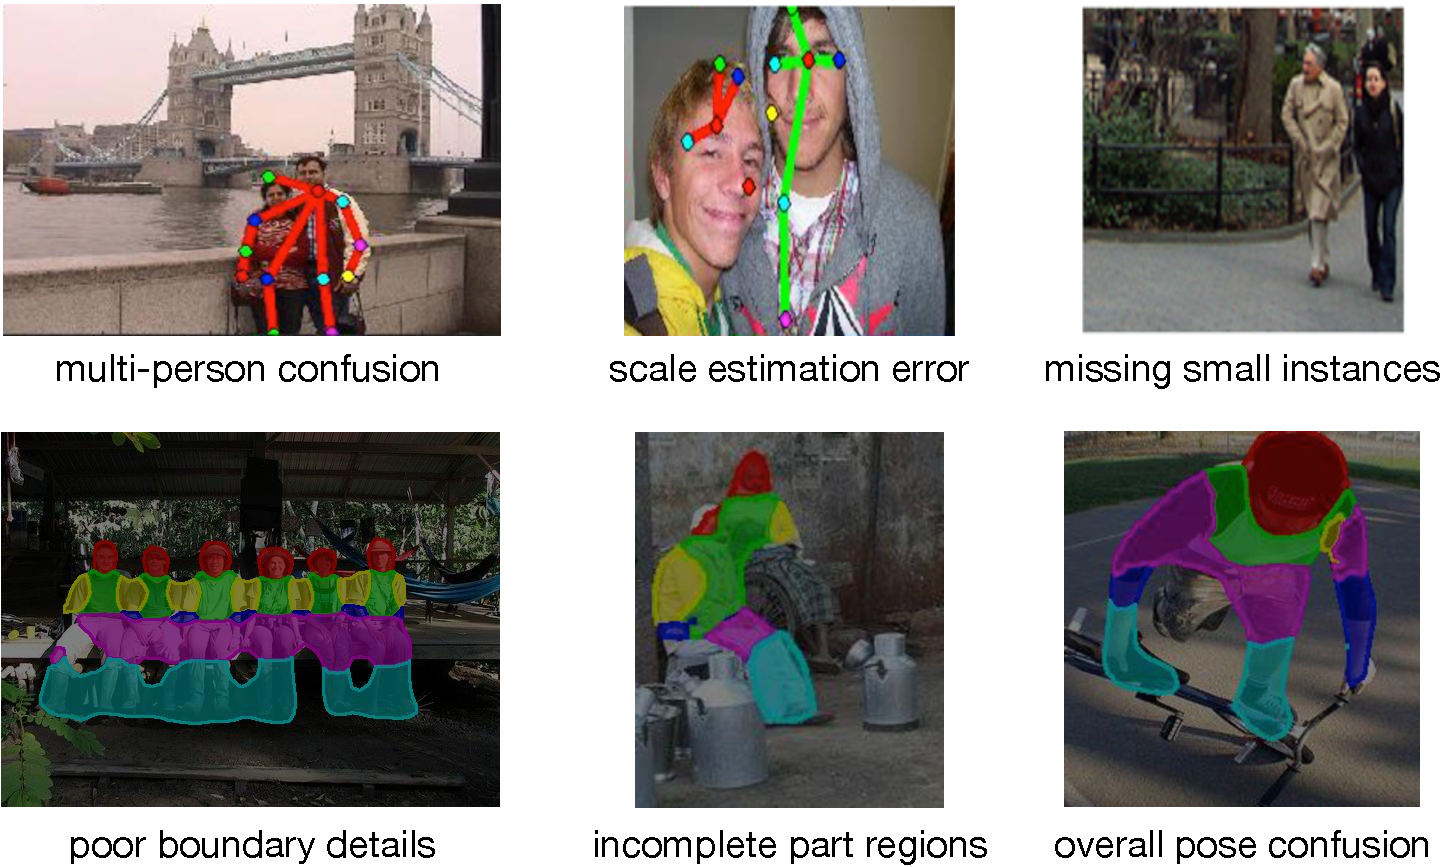
\includegraphics[width=1.0\linewidth]{figs/intro_hard.pdf}
\caption{Challenges for current human pose estimation algorithms (top row) and semantic part segmentation algorithms (bottom row) in natural multi-person scenes.}
\label{fig:challenge}
\end{figure}

\begin{figure*}
\begin{center}
 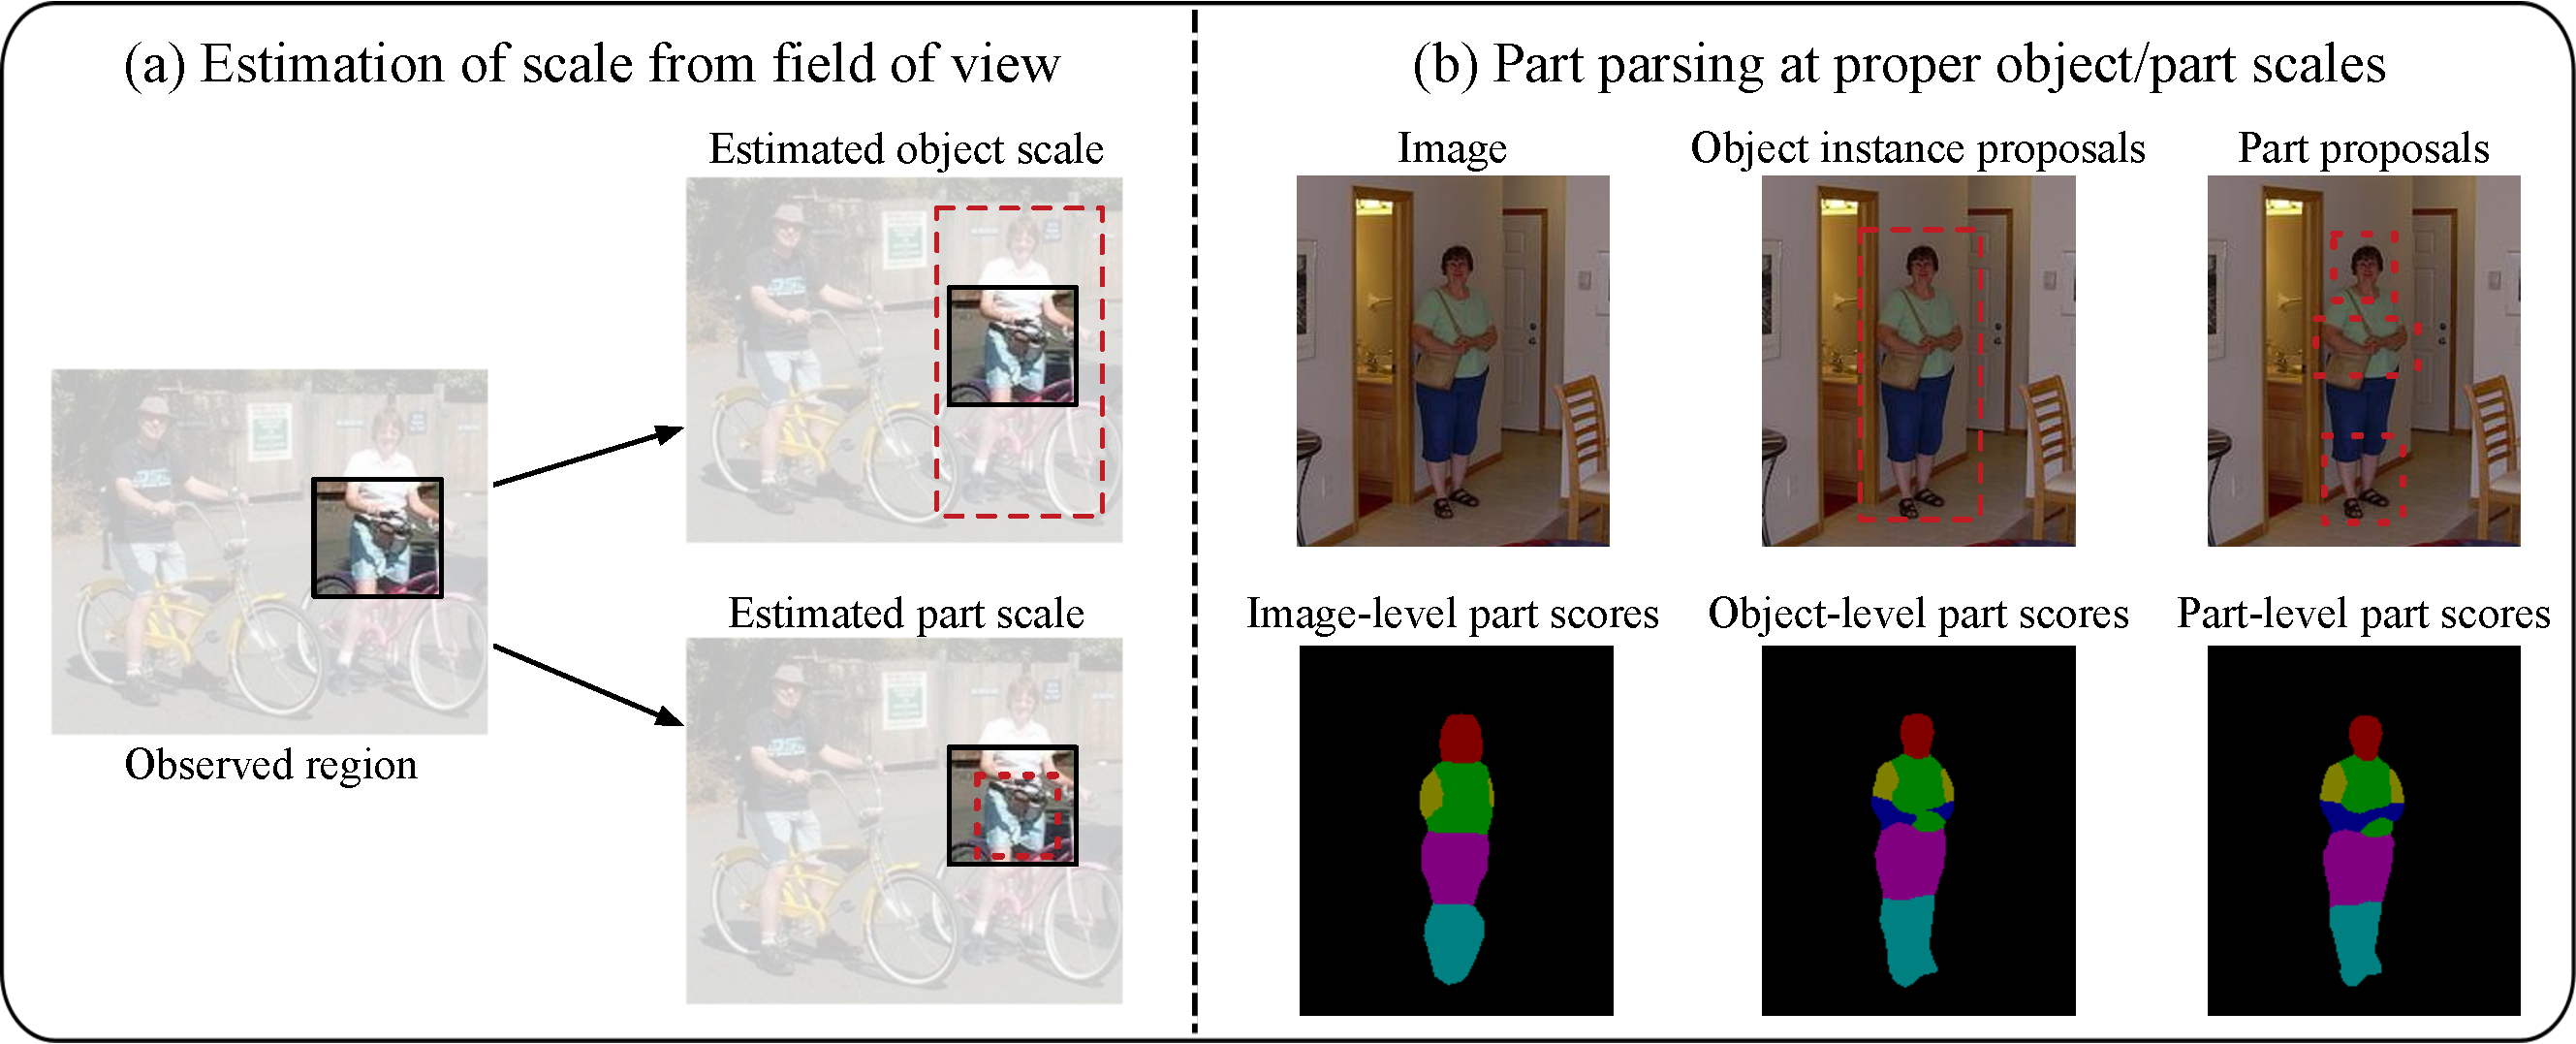
\includegraphics[width=0.8\textwidth]{figs/intuition_eccv.pdf}
\end{center}
\caption{Intuition of our hierarchical auto-zoom model (HAZN), which handles the large variation of object and part scale in natural multi-person scenes. (a) The scale
and location of an object and its parts (the red dashed boxes) can be estimated
from the observed field of view (the black solid box) of a neural network. (b)
Part segmentation can be more accurate by using proper object and part scales. In the top row, we show our estimated object and part scales. In the bottom row,
our part segmentation results gradually become better by increasingly utilizing the
estimated object and part scales.}
\label{fig:motivation_eccv}
\end{figure*}

% Difficulty of both tasks. Current methods and their shortcomings.
Currently, both semantic part segmentation and pose estimation face unsolved challenges in natural multi-person scenes (see Fig.~\ref{fig:challenge}).
Traditional semantic part segmentation methods~\cite{bo2011shape,eslami2012generative,yamaguchi2012parsing,dong2013deformable,zhu2011max} usually generate part segment proposals first and then use graphical models to select and assemble the part segment proposals into human instances. These methods are often time-consuming and only work well in constrained scenes, which pre-suppose known scale, fairly accurate localization, clear appearances, and/or relatively simple poses. Recently, dramatic progress has been made in semantic part segmentation due to the advent of fully convolutional neural networks (FCNs)~\cite{long2015fully} and the availability of object part annotations in large-scale datasets like PASCAL~\cite{chen2014detect}. These FCN-based methods~\cite{hariharan2015hypercolumns,wang2015joint,chen2016deeplab} usually compute pixel-wise part labels directly in a simple and fast way, and then optionally refine the labels by a graphical model such as the dense CRF~\cite{krahenbuhl2011efficient}. Although these FCN-based methods work well generally, they still suffer from the following two problems when handling natural multi-person scenes. They can make mistakes (e.g. missing small instances, producing poor boundary details or incomplete part regions, etc.) on small scale or extra large scale human instances for short of an effective mechanism to adapt to the size of the object instance. They also tend to produce erroneous predictions when the human instance is in an unusual pose or the appearance cues are weak, due to lack of object-level shape prior to regularize the part segments.

Similar to the trend of semantic part segmentation, traditional pose estimation approaches adopt graphical models to combine spatial constraints with local observations of joints, based on low-level features, like color intensities, HOG~\cite{dalal2005histograms}, shape-context~\cite{belongie2001shape}, and so on. Recent strategies rely on deep-learned joint detectors, and use a carefully designed graphical model to select and assemble joints into valid pose
configurations. Traditional approaches suffer from limited feature representation power and can only work in simple datasets with small pose and scale variation. Recent deep-based approaches have much better invariance to pose/scale variation, but their localization of joints is still inaccurate (e.g. joints are sometimes outside the human body) and they still struggle in multi-person overlapping scenes.

% Two main models in our framework.
In this paper, we present a scale-aware and pose-guided part segmentation framework that effectively improves human semantic part segmentation in natural images with large pose/scale variation. The framework mainly contains two novel models: (1) a hierarchical auto-zoom model (HAZN) that handles the large scale variation of human instances and human parts; (2) a joint prediction model that combines pose estimation and semantic part segmentation together, letting the two tasks benefit each other. Here we give a brief introduction to the two proposed models.

% Intuition of HAZN
The hierarchical "auto-zoom" model (HAZN) model is a FCN-based model performing object/part scale estimation and part segmentation at the same time, adapting to the size of objects and parts. It's partially motivated by the proposal-free end-to-end detection strategies~\cite{huang2015densebox,liang2015proposal,ren2015faster,redmon2016you}. To get some intuition of this approach, observe in Fig.~\ref{fig:motivation_eccv}(a), that the scale and location of a target object, and of its corresponding
parts, can be estimated accurately from the field-of-view (FOV) window
by applying a deep neural network. Using estimated object and part scales, the semantic part segmentation results can become better and better, see Fig.~\ref{fig:motivation_eccv}(b). Please refer to Sec.~\ref{sec:hazn} for a detailed explanation of the HAZN model. 

\begin{figure}
 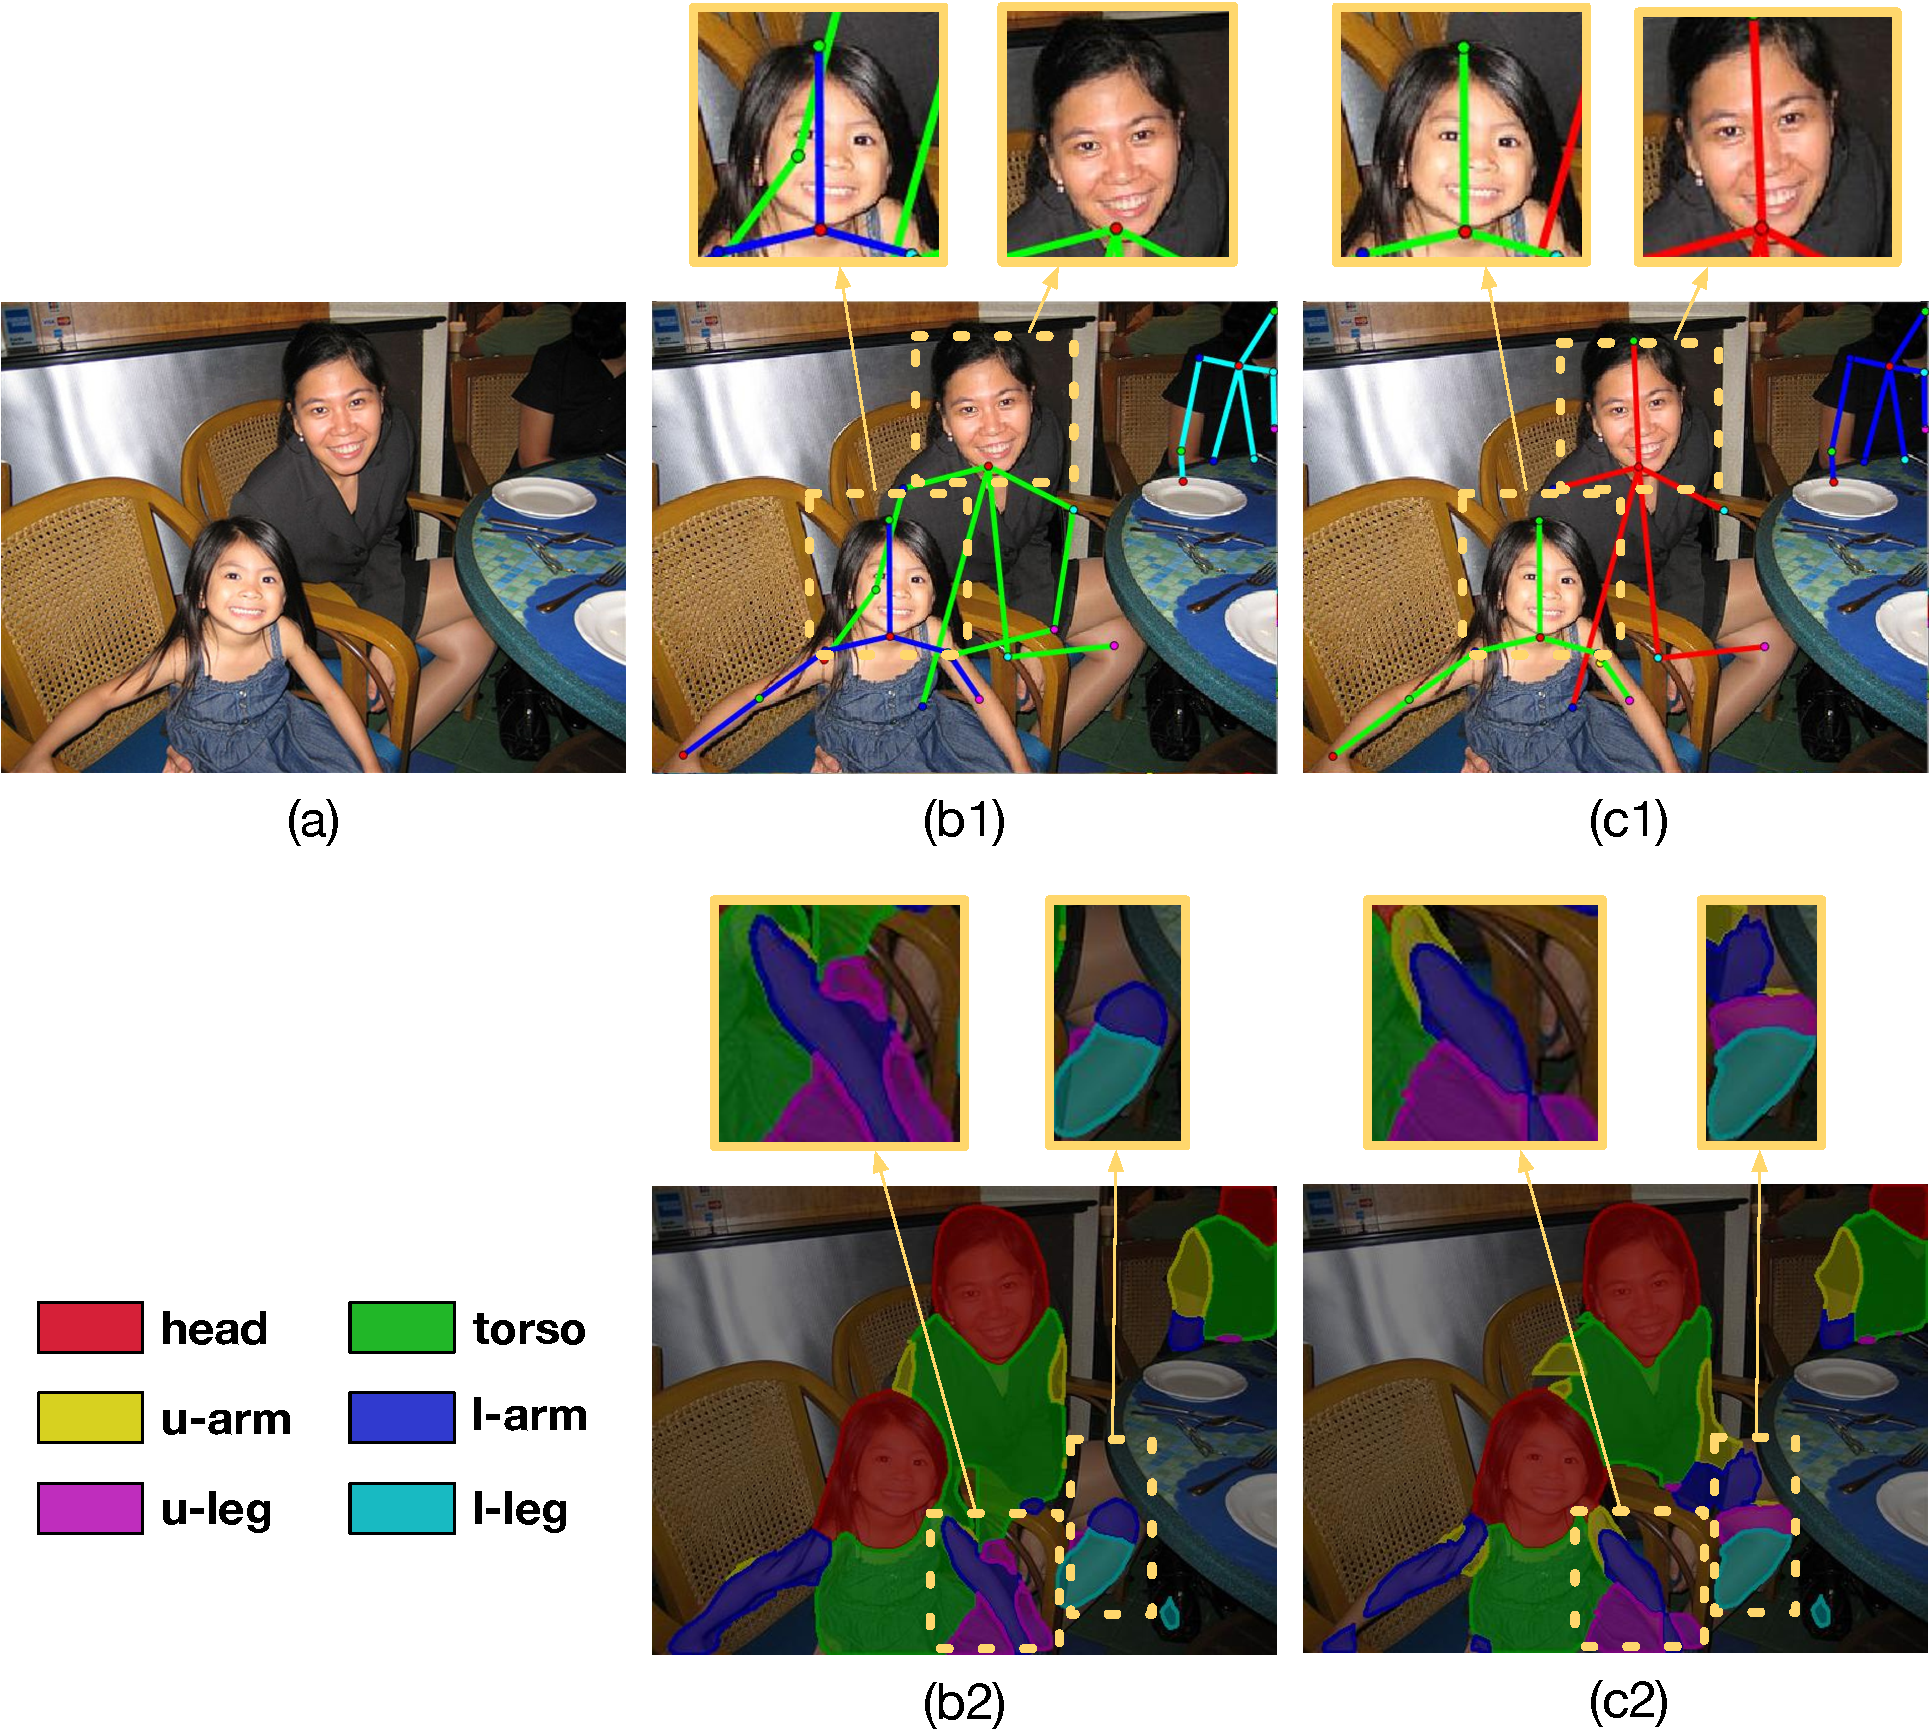
\includegraphics[width=1.0\linewidth]{figs/intuition_cvpr.pdf}
\caption{Joint human pose estimation and semantic part segmentation improve both tasks. (a) input image. (b) pose estimation and semantic part segmentation results before joint inference. (c) pose estimation and semantic part segmentation results after joint inference. Note that comparing (b1) and (c1), our result recovers the missing forehead joint and corrects the location error of right elbow and right wrist for the woman on the right. Comparing (b2) and (c2), our result gives more accurate details of lower arms and upper legs than (b2) for both people.}
\label{fig:motivation_cvpr}
\end{figure}

% Intuition of joint prediction model.
The joint prediction model is also a FCN-based framework aiming to solve the pose estimation task and the semantic part segmentation task jointly, in which the estimated pose provides object-level shape prior to regularize part segments (e.g. helping part segments align with human instances over the details of arms and legs where appearance cues are missing) while the part-level segments constrain the variation of pose locations (e.g. helping pose joints locate within their corresponding part segments). As shown in Fig.~\ref{fig:motivation_cvpr}, by taking advantage of the complementary property between pose estimation and semantic part segmentation, this joint prediction model produces better results on both tasks. See Sec.~\ref{sec:pose_and_seg} for detailed introduction of the model.

% Evaluation dataset and experiments.
In this paper, we address the task of human semantic part segmentation in ``the wild" where there are large variations in scale, pose, location, and occlusion. This motivates us to work with PASCAL images~\cite{everingham2014pascal} because these were chosen for studying multiple visual tasks, do not suffer from dataset design bias~\cite{li2014secrets}, and include large variations of objects, particularly of scale and pose. Hence human semantic part segmentation in PASCAL is considerably more difficult than in datasets, such as Fashionista~\cite{yamaguchi2012parsing}, that were constructed solely to evaluate human parsing. 

We illustrate our approach by extensive experiments on PASCAL-Person-Part dataset~\cite{chen2014detect}, which contains detailed part annotations for every person in a subset of PASCAL VOC 2010. We further augment this dataset with 14 pose joint locations through manual labeling to evaluate our joint prediction model. Our experiments show that our approach outperforms previous state-of-the-art methods for both semantic part segmentation and pose estimation tasks. We are particularly good at recovering small human parts, giving clearer details of arms and legs, and correcting local confusions of people.

\section{Related Works}
As human semantic part segmentation and human pose estimation are two fundamental topics in computer vision, many graphical models on the two topics have been proposed during the past thirty years. With the advent of powerful deep learning techniques, some models start to use deep-learned features, or even perform the whole task within a deep neural network. Recently, there are also works that combine pose estimation and segmentation in graphical models. In this section, we give an overall review of previous literature in these aspects.

\subsection{Human Semantic Part Segmentation}
% Traditional methods on human semantic part segmentation fall into two major categories. One type of methods first generate region/segment proposals for each semantic part, then select and assemble the region proposals by a graphical model. Bo et al.~\cite{bo2011shape} generated region proposals by UCM segmentation~\cite{arbelaez2009contours}, ranked the region proposals using shape and appearance features, and assembled the proposals with simple geometric constraints. \cite{dong2013deformable} got region proposals by UCM and CPMC~\cite{carreira2012cpmc}, extracted a rich set of appearance features for each region proposal encoded by Fisher Kernel and second-order pooling, and assembled the region proposals with a dedicated And-Or graph (AOG). The other type of methods treat semantic part segmentation as scene parsing, adopting pixel-wise conditional random fields (CRFs) to infer the pixel-wise part labels. \cite{Yamaguchi12_ParsingClothFashion} built a CRF based on super-pixels and tried to classify each super-pixel into one of the semantic part types. They learned unary part classifiers for super-pixels based on traditional features, and used the output scores as unary terms in the CRF. For the pairwise terms, they trained logistic regression models to predict whether two neighboring pixels should have the same label, and also learned a consistency prior between each part type pair from the training data. These traditional methods perform well on simple images, but struggle in natural images with large pose/scale variation.

\subsection{Human Pose Estimation}

\subsection{Joint Pose Estimation and Part Segmentation}

\section{Hierarchical Auto-Zoom Net}
\label{sec:hazn}

\section{Joint Prediction of Pose Estimation and Semantic Part Segmentation}
\label{sec:pose_and_seg}

\begin{acknowledgements}
AAA
\end{acknowledgements}

% BibTeX users please use one of
%\bibliographystyle{spbasic}      % basic style, author-year citations
%\bibliographystyle{spmpsci}      % mathematics and physical sciences
%\bibliographystyle{spphys}       % APS-like style for physics
%\bibliography{ijcv.bib}   % name your BibTeX data base

\begin{thebibliography}{}
%
% and use \bibitem to create references. Consult the Instructions
% for authors for reference list style.
%
%\bibitem{RefJ}
% Format for Journal Reference
%Author, Article title, Journal, Volume, page numbers (year)
% Format for books
%\bibitem{RefB}
%Author, Book title, page numbers. Publisher, place (year)
%
% Semantic part segmentation
\bibitem{rauschert2012generative}
Rauschert, Ingmar, and Robert T. Collins. "A generative model for simultaneous estimation of human body shape and pixel-level segmentation." In European Conference on Computer Vision, pp. 704-717 (2012)
\bibitem{long2015fully}
Long, Jonathan, Evan Shelhamer, and Trevor Darrell. "Fully convolutional networks for semantic segmentation." In Proceedings of the IEEE Conference on Computer Vision and Pattern Recognition (CVPR), pp. 3431-3440 (2015)
\bibitem{wang2015joint}
Wang, Peng, Xiaohui Shen, Zhe Lin, Scott Cohen, Brian Price, and Alan L. Yuille. "Joint object and part segmentation using deep learned potentials." In Proceedings of the IEEE International Conference on Computer Vision, pp. 1573-1581 (2015)
\bibitem{chen2016deeplab}
Chen, Liang-Chieh, George Papandreou, Iasonas Kokkinos, Kevin Murphy, and Alan L. Yuille. "Deeplab: Semantic image segmentation with deep convolutional nets, atrous convolution, and fully connected crfs." arXiv preprint arXiv:1606.00915 (2016)
\bibitem{bo2011shape}
Bo, Yihang, and Charless C. Fowlkes. "Shape-based pedestrian parsing." In Proceedings of the IEEE Conference on Computer Vision and Pattern Recognition (CVPR), pp. 2265-2272 (2011)
\bibitem{eslami2012generative}
Eslami, S., and Christopher Williams. "A generative model for parts-based object segmentation." In Advances in Neural Information Processing Systems (NIPS), pp. 100-107 (2012)
\bibitem{yamaguchi2012parsing}
Yamaguchi, Kota, M. Hadi Kiapour, Luis E. Ortiz, and Tamara L. Berg. "Parsing clothing in fashion photographs." In Proceedings of the IEEE Conference on Computer Vision and Pattern Recognition (CVPR), pp. 3570-3577 (2012)
\bibitem{dong2013deformable}
Dong, Jian, Qiang Chen, Wei Xia, Zhongyang Huang, and Shuicheng Yan. "A deformable mixture parsing model with parselets." In International Conference on Computer Vision (ICCV), pp. 3408-3415 (2013)
\bibitem{zhu2011max}
Zhu, Long Leo, Yuanhao Chen, Chenxi Lin, and Alan Yuille. "Max margin learning of hierarchical configural deformable templates (hcdts) for efficient object parsing and pose estimation." In International Journal of Computer Vision, 93(1), pp 1-21 (2011)
\bibitem{hariharan2015hypercolumns}
Hariharan, Bharath, Pablo Arbeláez, Ross Girshick, and Jitendra Malik. "Hypercolumns for object segmentation and fine-grained localization." In Proceedings of the IEEE Conference on Computer Vision and Pattern Recognition (CVPR), pp. 447-456 (2015)
\bibitem{krahenbuhl2011efficient}
Krähenbühl, Philipp, and Vladlen Koltun. "Efficient inference in fully connected crfs with gaussian edge potentials." In Advances in Neural Information Processing Systems (NIPS), pp. 109-117 (2011)
%
% Pose estimation
\bibitem{yang2011articulated}
Yang, Yi, and Deva Ramanan. "Articulated pose estimation with flexible mixtures-of-parts." In Proceedings of the IEEE Conference on Computer Vision and Pattern Recognition (CVPR), pp. 1385-1392 (2011).
\bibitem{tompson2015efficient}
Tompson, Jonathan, Ross Goroshin, Arjun Jain, Yann LeCun, and Christoph Bregler. "Efficient object localization using convolutional networks." In Proceedings of the IEEE Conference on Computer Vision and Pattern Recognition (CVPR), pp. 648-656 (2015)
\bibitem{chen2015parsing}
Chen, Xianjie, and Alan Yuille. "Parsing occluded people by flexible compositions." In Proceedings of the IEEE Conference on Computer Vision and Pattern Recognition (CVPR), pp. 3945-3954 (2015)
%
% Fine-grained recognition
\bibitem{branson2014bird}
Branson, Steve, Grant Van Horn, Serge Belongie, and Pietro Perona. "Bird species categorization using pose normalized deep convolutional nets." arXiv preprint arXiv:1406.2952 (2014)
\bibitem{zhang2014part}
Zhang, Ning, Jeff Donahue, Ross Girshick, and Trevor Darrell. "Part-based R-CNNs for fine-grained category detection." In European Conference on Computer Vision, pp. 834-849 (2014)
\bibitem{krause2016unreasonable}
Krause, Jonathan, Benjamin Sapp, Andrew Howard, Howard Zhou, Alexander Toshev, Tom Duerig, James Philbin, and Li Fei-Fei. "The unreasonable effectiveness of noisy data for fine-grained recognition." In European Conference on Computer Vision, pp. 301-320 (2016)
%
% Action recognition
\bibitem{wang2012discriminative}
Wang, Yang, Duan Tran, Zicheng Liao, and David Forsyth. "Discriminative hierarchical part-based models for human parsing and action recognition." In Journal of Machine Learning Research, 13(Oct), pp. 3075-3102 (2012)
\bibitem{zhou2015interaction}
Zhou, Yang, Bingbing Ni, Richang Hong, Meng Wang, and Qi Tian. "Interaction part mining: A mid-level approach for fine-grained action recognition." In Proceedings of the IEEE Conference on Computer Vision and Pattern Recognition (CVPR), pp. 3323-3331 (2015)
\bibitem{chunyu_action}
Wang, Chunyu, Yizhou Wang, and Alan L. Yuille. "An approach to pose-based action recognition." In Proceedings of the IEEE Conference on Computer Vision and Pattern Recognition (CVPR), pp. 915-922 (2013)
%
% Person identification
\bibitem{ma2011human}
Ma, Lianyang, Xiaokang Yang, Yi Xu, and Jun Zhu. "Human identification using body prior and generalized EMD." In Image Processing (ICIP) 18th IEEE International Conference, pp. 1441-1444 (2011)
\bibitem{zhao2017deeply}
Zhao, Liming, Xi Li, Jingdong Wang, and Yueting Zhuang. "Deeply-learned part-aligned representations for person re-identification." arXiv preprint arXiv:1707.07256 (2017)
%
% Video surveillance
\bibitem{gallego2008segmentation}
Gallego, Jaime, Montse Pardas, and Jose-Luis Landabaso. "Segmentation and tracking of static and moving objects in video surveillance scenarios." In Image Processing (ICIP) 15th IEEE International Conference, pp. 2716-2719 (2008)
\bibitem{liu2017surveillance}
Liu, Si, Changhu Wang, Ruihe Qian, Han Yu, Renda Bao, and Yao Sun. "Surveillance video parsing with single frame supervision." In IEEE Conference on Computer Vision and Pattern Recognition (CVPR) workshops, pp. 1-9 (2017)
% 
% Object Detection
\bibitem{huang2015densebox}
Huang, Lichao, Yi Yang, Yafeng Deng, and Yinan Yu. "Densebox: Unifying landmark localization with end to end object detection." arXiv preprint arXiv:1509.04874 (2015)
\bibitem{liang2015proposal}
Liang, Xiaodan, Yunchao Wei, Xiaohui Shen, Jianchao Yang, Liang Lin, and Shuicheng Yan. "Proposal-free network for instance-level object segmentation." arXiv preprint arXiv:1509.02636 (2015)
\bibitem{ren2015faster}
Ren, Shaoqing, Kaiming He, Ross Girshick, and Jian Sun. "Faster r-cnn: Towards real-time object detection with region proposal networks." In Advances in Neural Information Processing Systems (NIPS), pp. 91-99 (2015)
\bibitem{redmon2016you}
Redmon, Joseph, Santosh Divvala, Ross Girshick, and Ali Farhadi. "You only look once: Unified, real-time object detection." In Proceedings of the IEEE Conference on Computer Vision and Pattern Recognition (CVPR), pp. 779-788 (2016)
%
% Dataset
\bibitem{chen2014detect}
Chen, Xianjie, Roozbeh Mottaghi, Xiaobai Liu, Sanja Fidler, Raquel Urtasun, and Alan Yuille. "Detect what you can: Detecting and representing objects using holistic models and body parts." In Proceedings of the IEEE Conference on Computer Vision and Pattern Recognition (CVPR), pp. 1971-1978 (2014)
%
% Background
\bibitem{dalal2005histograms}
Dalal, Navneet, and Bill Triggs. "Histograms of oriented gradients for human detection." In Proceedings of the IEEE Conference on Computer Vision and Pattern Recognition (CVPR), pp. 886-893 (2005)
\bibitem{belongie2001shape}
Belongie, Serge, Jitendra Malik, and Jan Puzicha. "Shape context: A new descriptor for shape matching and object recognition." In Advances in Neural Information Processing Systems (NIPS), pp. 831-837 (2001)
\bibitem{everingham2014pascal}
Everingham, Mark, SM Ali Eslami, Luc Van Gool, Christopher KI Williams, John Winn, and Andrew Zisserman. "The pascal visual object classes challenge: A retrospective." In International Journal of Computer Vision 111, no. 1, pp 98-136 (2015)
\bibitem{li2014secrets}
Li, Yin, Xiaodi Hou, Christof Koch, James M. Rehg, and Alan L. Yuille. "The secrets of salient object segmentation." In Proceedings of the IEEE Conference on Computer Vision and Pattern Recognition (CVPR), pp. 280–287 (2014)
\end{thebibliography}

\end{document}
% end of file template.tex

